\documentclass{sigchi}

% Remove or comment out these two lines for final version
\toappear{ Permission to make digital or hard copies of all or part of
  this work for personal or classroom use is granted without fee
  provided that copies are not made or distributed for profit or
  commercial advantage and that copies bear this notice and the full
  citation on the first page. To copy otherwise, or republish, to post
  on servers or to redistribute to lists, requires prior specific
  permission and/or a fee.

Gamification'13, October 2-4, 2013, Stratford, ON, Canada.

Copyright 2013 ACM 978-1-XXXX-XXXX-X/XX/XX...\$10.00.
}

\pagenumbering{arabic}% Arabic page numbers for submission. 

% Use \toappear{...} to override the default ACM copyright statement (e.g. for preprints).

% Load basic packages
\usepackage{balance}  % to better equalize the last page
\usepackage{graphicx} % for EPS, load graphicx instead
\usepackage{times}    % comment if you want LaTeX's default font
\usepackage{url}      % llt: nicely formatted URLs
\usepackage{paralist} % compact lists


\usepackage{subfigure}
\graphicspath{{figures/}}

% llt: Define a global style for URLs, rather that the default one
\makeatletter
\def\url@leostyle{%
  \@ifundefined{selectfont}{\def\UrlFont{\sf}}{\def\UrlFont{\small\bf\ttfamily}}}
\makeatother
\urlstyle{leo}

% To make various LaTeX processors do the right thing with page size.
\def\pprw{8.5in}
\def\pprh{11in}
\special{papersize=\pprw,\pprh}
\setlength{\paperwidth}{\pprw}
\setlength{\paperheight}{\pprh}
\setlength{\pdfpagewidth}{\pprw}
\setlength{\pdfpageheight}{\pprh}

%% Puts space after macros, unless followed by punctuation
\usepackage{xspace}

%%% Personal macros
%% Tired of typing CO2 so many times, requires xspace package
\newcommand{\COtwo}{CO\ensuremath{_2}\xspace}
%% Hawai`i with okina
\newcommand{\Hawaii}{Hawai`i\xspace}
%% Hawai`ian with okina
\newcommand{\Hawaiian}{Hawai`ian\xspace}
%% Manoa with kahako
\newcommand{\Manoa}{M\=anoa\xspace}

% Make sure hyperref comes last of your loaded packages, 
% to give it a fighting chance of not being over-written, 
% since its job is to redefine many LaTeX commands.
\usepackage[dvips]{hyperref}
\hypersetup{
pdftitle={Serious Game Framework Evaluation: A Case Study of Makahiki},
pdfauthor={LaTeX},
pdfkeywords={SIGCHI, proceedings, archival format},
bookmarksnumbered,
pdfstartview={FitH},
colorlinks,
citecolor=black,
filecolor=black,
linkcolor=black,
urlcolor=black,
breaklinks=true,
}

%% Make links to captions point to the figure, not just the caption at bottom
\usepackage[all]{hypcap}

% create a shortcut to typeset table headings
\newcommand\tabhead[1]{\small\textbf{#1}}

%% Since I'm using the LaTeX Makefile that uses dvips, I need this
%% package to make URLs break nicely
\usepackage{breakurl}

% End of preamble. Here it comes the document.
\begin{document}

\title{SGSEEM: Evaluating Serious Game Frameworks\\ from a Stakeholder Experience Perspective}

% Note that submissions are blind, so author information should be omitted
%\numberofauthors{5}
%\author{
%  \alignauthor Yongwen Xu, Philip M. Johnson, Carleton A. Moore, Robert S. Brewer, Jordan Takayama\\
%    \affaddr{Department of Information and Computer Sciences}\\
%    \affaddr{University of Hawaii at Manoa}\\
%    \affaddr{Honolulu, HI, USA}\\
%    \email{\{yxu, johnson, cmoore, rbrewer, jktakaya\}@hawaii.edu}\\
%}

\maketitle

\begin{abstract}
% 150 words max
  There is little research or experience with formal evaluation of serious game
  frameworks. To fill this gap, this paper describes an evaluation mechanism called the
  Serious Game Stakeholder Experience Evaluation Method (SGSEEM). SGSEEM is designed to
  provide detailed insights into the strengths and weaknesses of serious game frameworks
  through a stakeholder perspective based approach.

  In this paper, we report on the use of SGSEEM to evaluate
  Makahiki, an open source serious game framework for sustainability.  Makahiki 
  facilitates the development of serious games for the purpose of education and
  behavioral change regarding energy and water consumption. Makahiki and SGEEM together
 provide useful insights into the challenges and opportunities of serious game framework design and evaluation.
\end{abstract}

\keywords{
	serious games; framework evaluation; sustainability
}

\category {H.5.m.} {Information Interfaces and Presentation (e.g., HCI)} {Miscellaneous} {K.8.0.} {Personal Computing} {Games}

%\\
%\textcolor{red}{See: \url{http://www.acm.org/about/class/1998/}
%for more information and the full list of ACM classifiers and descriptors. 
%Mandatory section: On the submission page
%only the classifiers' letter-number combination will need to be entered.}


\terms{
	Serious Game; Evaluation; Game Design; Case study.
}

\section{Introduction}

Serious games (games with additional goals beyond just entertainment) have been the topic
of academic research for decades~\cite{Zyda2005}. Such games show great potential as
successful interactive media that provide engaging interfaces in various serious
contexts~\cite{mcgonigal2011reality,reeves2009total}. The recent phenomenon of
gamification~\cite{Deterding2011mt} also calls for game-related research in areas beyond
traditional entertainment purposes.

One of the fundamental questions in assessing a serious game is the extent to which the
game achieves its ``serious'' purpose.  This is quite different from 
traditional entertainment games, in which assessment focuses on usability or
playability~\cite{song2007new}. In the field of serious games, there is an increasing
focus on the methodology of research and evaluation~\cite{Mayer2012233}. De Freitas and
Oliver describe a four dimensional framework~\cite{de2006can} for evaluating an
educational game, consisting of: the context, the pedagogy, the representation, and the
learner (or player). Harteveld proposes an alternative approach called "Triadic Game
Evaluation"~\cite{harteveld2010triadic}, consisting of three perspectives: Reality,
Meaning, and Play.

The above approaches focus on evaluation of a single game, as opposed to a game {\em
  framework}. Game frameworks (also known as game engines) are ``comprised of a collection
of different tools, utilities, and interfaces that hide the low-level details of the
various tasks that make up a game''~\cite{sherrod2006ultimate}. One of the benefits of
using a serious game framework is that, if correctly designed, it will provide useful and
reusable ``building blocks'' for a serious game.  These building blocks enable the serious
game developer to focus more time and thought on content and results instead of on
infrastructure.  Yet how are we to know if a serious game framework has been ``correctly designed''?

To help answer this question, this paper proposes a method for evaluating serious game
frameworks, called the Serious Game Stakeholder Experience Evaluation Method (SGSEEM). In
a nutshell, SGSEEM identifies the most important stakeholders of a serious game framework
and provides a method for gaining insight into the extent with which the framework is
effective and efficient with respect to each stakeholders' perspective.

To best understand SGSEEM, we will start by briefly introducing Makahiki, our serious game
framework for sustainability, and how its development motivated us to create the SGSEEM method. We then describe our preliminary
results from the application of SGSEEM to Makahiki. We conclude with the insights this
evaluation process provides for our own work on Makahiki as well as for serious game
design in general.


\section{Motivation for SGSEEM}

Sustainability education and conservation have become an international
imperative due to the rising cost of energy, increasing scarcity of
natural resources, and irresponsible environmental practices. Over the
past decade, energy and water challenges have become focal
points for sustainability efforts at both university and industry
campuses. For example, college residence hall energy competitions have
been a widespread mechanism for engaging students in energy issues,
with more than 160 taking place or being planned for the 2010--2011
academic year in North America~\cite{Hodge2010}.

Designers of such challenges typically have three choices for
information technology support: (a) build their own custom in-house
solution (as was done at Oberlin College in
2006~\cite{petersen-dorm-energy-reduction}); (b) out-source to a
commercial provider (as was done at the University of British Columbia
in 2011); or (c) use a minimal tech solution such as a web page and
manual posting of data and results (as was done at Harvard in 2012).

None of these choices are ideal: the custom in-house solution requires
sophisticated design and implementation skills; out-sourcing can be
financially expensive and impedes evolution; and the minimal tech
solution does not fully leverage the possibilities of advanced
information technology.

To provide a better alternative to these three choices, we designed and implemented
an open source serious game framework for sustainability called
Makahiki~\cite{csdl2-12-06}.  Makahiki implements an extensible framework with a variety
of common services for developing sustainability games including: authentication; game
mechanics such as leaderboards, points, and badges; a variety of built-in games and
content focused on sustainability; a responsive user interface; cloud-based deployment;
and the ability to customize the game to the needs of individual organizations.  
Figure \ref{fig:Makahiki-Home-Page} illustrates a home page implemented using Makahiki.

\begin{figure}
  \center
  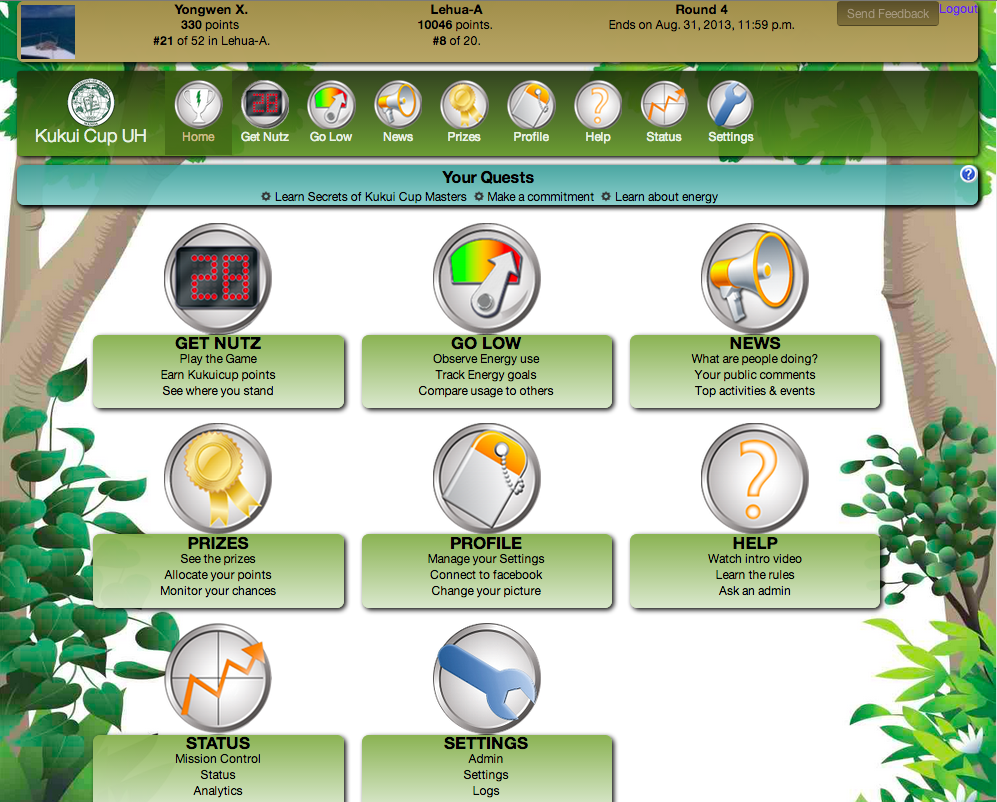
\includegraphics[width=\columnwidth]{kukuicup-home}
  \caption{Makahiki Game Instance}
  \label{fig:Makahiki-Home-Page}
\end{figure}

To explore the ability of the Makahiki framework to support
sustainability games in different environments, we ran three
challenges at different organizations in Fall 2012: The University of
Hawaii, Hawaii Pacific University, and the East-West Center. While
these experiences provided anecdotal evidence for the usefulness of
Makahiki as a framework, we realized that a more rigorous evaluation of the framework
would yield better insight into its current quality and requirements
for future enhancement.

Upon reviewing the literature, we found little prior work concerning formal evaluation for
the particular needs of serious game frameworks. As a result, we designed SGSEEM, and
began applying it to gain better insight into Makahiki as a result of its usage in three
game challenges during 2012.

\section{Serious Game Stakeholder Experience Evaluation Method (SGSEEM)}

The goal of SGSEEM is to determine to what extent the serious game
framework under evaluation, as an Information Technology (IT)
infrastructure, can effectively and efficiently support the
development and play of a serious game.

An \emph{effective} serious game framework can produce a game with the desired outcome
with respect to its ``serious'' goals for the players. For example, an effective serious
game framework for energy education and conservation produces a game that increases
players' energy literacy and reduces their energy consumption during (and, hopefully,
after) the game. Because the goals of serious games are always subject specific, the
desired effect of a serious game for sustainability is different than the desired effect
of a serious game for language learning, or for healthy eating.  In this paper, we will 
refer to subject-specific goals relevant to sustainability, but users of SGSEEM in other
domains will substitute goals for their area. 

An \emph{efficient} serious game framework can support the
full life cycle of game development, execution, and wrap-up of the
serious game, including design, management, administration, development,
and improvement of the game.

\subsection{Methodology}

% PJ:  Definitely need some references to mixed method evaluation approaches here. 
% See Chapter 5, section 1 for starters:
% https://csdl-techreports.googlecode.com/svn/trunk/techreports/2006/06-05/06-05.pdf
% This section needs more detail and more explanation of how it relates to other methods.

Creswell \cite{creswell2003} categorizes research methods into three approaches:
quantitative, qualitative, and mixed-methods, according to what constitutes knowledge
and how knowledge is best acquired. Derided from his work, SGSEEM is based upon the mixed-methods with both qualitative and quantitative data collection and analysis.

% PJ: More here on how SGSEEM methodology relates/uses qualitative/quantitative data
% analysis techniques.

In SGSEEM, qualitative analysis involves structured interviews and questionnaires to stakeholders designed to gain insight about their experiences with the
framework under study. Besides qualitative analysis, SGSEEM also employs quantitative analysis involving the analytical data recorded by the system, including website logs, player interaction logs, feedback, resource usage, etc.

\subsection{Stakeholders}

There are many more stakeholders in serious games than in traditional entertainment
games. The following are the stakeholders we identified for our sustainability serious game framework:

\begin{compactitem}
\item \emph{Players}: those who participate in the game play.
\item \emph{System Admins}: those who install and maintain the technological game infrastructure.
\item \emph{Game Designers}: those who design the content and game mechanics.
 \item \emph{Game Managers}: those who manage the game during the period of game play.
\item \emph{Developers}: those who extend, enhance and debug the game framework.
\item \emph{Researchers}: those who are conducting research using the game framework.
\item \emph{Spectators}: those who do not participate in the game
  play but are interested in the game and the results of game play.
\item \emph{Community partners}: those who partner
  with the game organizers to help run the game (such as coordinating real-world events as part of the game).
\item \emph{Facilities}: those who are responsible for the resources (energy, water, etc)
  associated with the game.
\item \emph{Funding organizations}: the organizations who provide
  funding to the project.
\end{compactitem}

The overall success of a serious game framework for sustainability depends on the
individual success of all of these stakeholders. However, as SGSEEM focuses on the software
infrastructure, it does address the spectator, community partner, facilities, and funding
organization stakeholders.  These are important stakeholders but outside the scope of our
evaluation method.

Our case study evaluation of Makahiki using SGSEEM evaluates (1) aspects of 
effectiveness of the system for Players, and (2) aspects of both effectiveness and
efficiency for Game Designers, Game Managers, System Admins, Developers, and Researchers. 

\autoref{fig:evaluation-framework} provides an overview of the evaluation framework. The
following sections describe in detail the evaluation mechanism for each stakeholder.

\begin{figure}
  \centering
  \begin{tabular}{|c|c|}
    \hline
    \multicolumn{1}{|p{0.3\columnwidth}|}{\centering\tabhead{Stakeholder}} &
    \multicolumn{1}{|p{0.65\columnwidth}|}{\centering\tabhead{Evaluation Goal}} \\
    \hline
    \multicolumn{1}{|p{0.3\columnwidth}|}{Players} &
    \multicolumn{1}{|p{0.65\columnwidth}|}{Effectiveness of the game
      to players in terms of literacy and behavior change in
      sustainability, player engagement} \\ 
    \hline
    \multicolumn{1}{|p{0.3\columnwidth}|}{System admins} & \multicolumn{1}{|p{0.65\columnwidth}|}{Efficiency in administrating the system} \\
    \hline
    \multicolumn{1}{|p{0.3\columnwidth}|}{Game designers} & \multicolumn{1}{|p{0.65\columnwidth}|}{Efficiency in designing a game} \\
    \hline
    \multicolumn{1}{|p{0.3\columnwidth}|}{Game managers} & \multicolumn{1}{|p{0.65\columnwidth}|}{Efficiency in managing a game} \\
    \hline
    \multicolumn{1}{|p{0.3\columnwidth}|}{Developers} & \multicolumn{1}{|p{0.65\columnwidth}|}{Efficiency in developing a game or enhancing the system} \\
    \hline
    \multicolumn{1}{|p{0.3\columnwidth}|}{Researchers} & \multicolumn{1}{|p{0.65\columnwidth}|}{Efficiency in performing research} \\
    \hline
  \end{tabular}
  \caption{Overview of SGSEEM}
  \label{fig:evaluation-framework}
\end{figure}

\subsubsection{1. Player Effectiveness}

SGSEEM assesses the ``effectiveness'' of a serious game framework for the
Player stakeholder by addressing three questions: (a) To what extent does the game
increase player's literacy in sustainability? (b) To what extent does
the game produce positive player behavior change in sustainability?
(c) To what extent does the game engage players?

\autoref{fig:pre-post-eval} illustrates the process for player
effectiveness evaluation, which involves a pre-game and post-game
measurement for literacy and behavior change, as well as the in-game
data logging to measure the level of player engagement.

\begin{figure}
  \center
  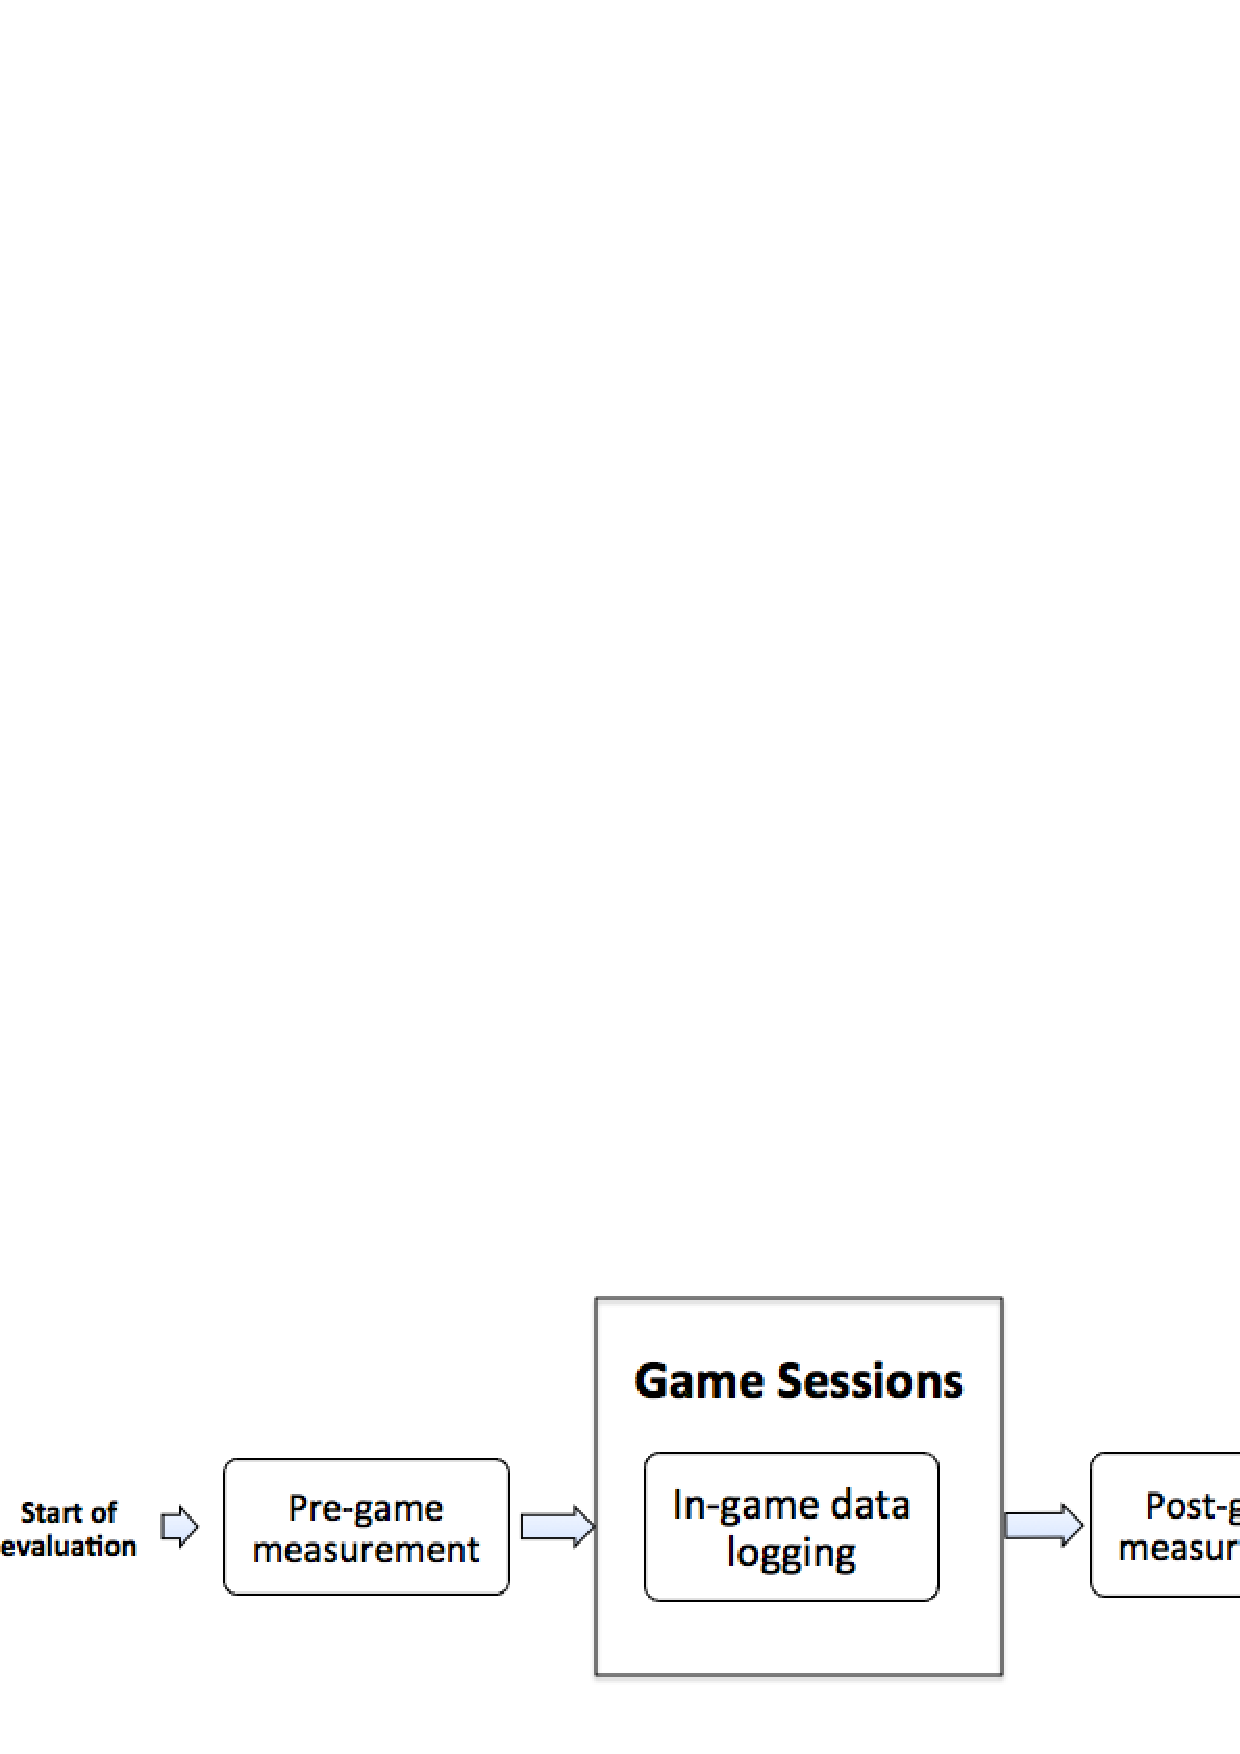
\includegraphics[width=\columnwidth]{pre-post-eval}
  \caption{Player Effectiveness Evaluation Process}
  \label{fig:pre-post-eval}
\end{figure}

\emph {(a) Literacy assessment:} One important goal of a serious
game for sustainability is to produce a change in knowledge in the
players. A literacy assessment can indicate whether this goal is being met.

SGSEEM uses an approach similar to that described in \cite{csdl2-10-08} to
assess the impact of the game on player literacy. In general, a set of literacy survey
questionnaires are presented to a random selection of the players 
before the game. After the game ends, the same survey
(post-game) is presented to the players who responded the
pre-game survey. These two set of survey response data are
compared to understand if the game has had an impact on literacy.

The extent of players' sustainability literacy change will indicate
the degree of educational effectiveness of the serious game for
sustainability.

\emph {(b) Behavior change assessment:} Positive behavior change is
another main goal of a serious game for sustainability. A serious game
for sustainability may include some degree of resource
consumption measurement. SGSEEM uses resource consumption data before and
after the game as part of the assessment of the
players' sustainability behavior change.  A resource consumption
baseline can be established based on historical
consumption data. During and after the game, we can compare the
resource consumption with the baseline for a particular day to
understand to what extent the resource consumption has changed.

The problems with using a baseline to assess the energy reduction in the case of dormitory
energy challenges is discussed in detail by Johnson et al.~\cite{csdl2-12-08}. As a method
for evaluating the effectiveness of serious game for sustainability in a broader context
beyond the dormitory challenge, we continue to use the baseline method as one way to
assess changes in resource consumption.

In addition to resource consumption, SGSEEM can include the use of a
behavior survey to measure self-reported behavior
change. A pre-game survey is be presented to the players to ask about
their current sustainability behavior, then after the game, a post-game
survey is presented to ask about the players' behavior again. These two
sets of survey response data can be compared to understand if there is
any changes.

The combination of resource consumption changes and self-reported
behavior changes can be used to assess the degree of behavior
effectiveness of the serious game for sustainability.

\emph {(c) Engagement assessment:} Player engagement is an important measure for
understanding the effectiveness of a serious game. By investigating the degree of
engagement, we can determine to what extent individuals are participating in the game, as
well as to what extent the community population is participating in the game.

%% PJ: Note that I rewrote the following paragraph!

Engagement has a subtle relationship to the overall effectiveness of a serious game. It is
possible for the game to be played by only a subset of the target population, but
have an impact on those not playing by virtue of their contact with players. Gaining 
better insight into this effect is an area of active study for us. 

To obtain engagement data, SGSEEM requires the framework to support the following measures
based upon system log data: 

\begin{compactitem}
\item participation rate
\item number of players per day
\item play time of a player per day
\item submissions of all player per day
\item social interaction of all player per day
\item website errors per day
\end{compactitem}

%PJ include a paragraph saying how this data is analyzed.
The participation rate measures the percentage of users who used the game system based on the total eligible players. In the serious game context, it indicates the level of involvement or awareness of the serious matters. The number of players and play time per day measure how frequently the players interact with the game system. The submissions per day measures the rate of serious game specific activities (online or real world) players completed, while the social interaction per day measures the rate of any social interaction between the players. At last, the website errors per day measures the rate of errors encountered by the players. In general, with the opposite of website error measurement, the higer value of these measurements are, the higher engagement level the system has.

\subsubsection{2. System Admin Efficiency}

System administrators simply install the framework and dependent libraries, do backups,
and so forth. SGSEEM assesses the efficiency of the system admin stakeholder through
interviews involving the following questions:

\begin{compactitem}
\item How much time did you require to install the system, including the dependency?
\item How much time did you require to maintain the system?
\item What problems did you encounter?
\item Did you find it difficult to admin the system? What was difficult?
\item What did you like the least about administering the system?
\end{compactitem}

%PJ include a paragraph saying how this data is analyzed.
After the interview data is acquired, the evaluator will perform qualitative data
analysis, which involves transcribing (if the interview data is in audio format),
categorizing and coding the problem or difficulty description. Once the categories of
 problems are coded, the evaluator could analyze the time and problem they reported
 to identify the area of strength (less time spent) and weakness (problems and
 difficulties).

\subsubsection{3. Game Designer Efficiency}

SGSEEM measures the efficiency of a serious game framework with respect to the Game
Designer stakeholder by addressing the following two questions: (a) How much time is
required to design an instance of a serious game using the framework? and (b) How many,
and how problematic are the errors that designers encounter during the design process?

A serious game framework always provides certain tools or interfaces to game designers
with the hope that these will simplify the design of a game. Such tools might involve
configuring global settings for the game, such as how long will the game run, who are the
players, and how to design individual game elements.

SGSEEM requires the evaluator to first identify the sequence of tasks to be carried out by
the Game Designer, then acquire two sets of assessment data.
The first dataset is the system log data for the interaction between the game designer
and the serious game framework. This data can help determine how much 
time it takes a designer to complete a certain design task using the game
framework, and any errors encountered. 

A second set of data is obtained by interviewing the designer and asking the following questions:
\begin{compactitem}
\item How much time did you spend to complete each design task?
\item What problems did you encounter?
\item Did you find it difficult to configure? What was difficult?
\item Did you find it difficult to design a specific game? Which one, and what was difficult?
\item What did you like the least when using the system?
\end{compactitem}

%PJ include a paragraph saying how this data is analyzed.
The interview data will also be transcribed (if audio recording), categorised, coded. The time data from the interviews will be validated by the system log data, while the descriptive problem categories will be correlated with the system log time and error data.

\subsubsection{4. Game Manager Efficiency}

SGSEEM measures the efficiency of a serious game framework with respect to the Game
Manager stakeholder with questions similar to those above: (a) How much time is
required to manage an instance of a serious game using the framework? and (b) How many,
and how problematic are the errors that managers encounter during the design process?

Serious game frameworks normally provide certain interfaces for the managers to manage the
game. This may involve managing player submissions, monitoring the game state, entering
manual resource data, notifying winners of the game, etc.

As before, SGSEEM requires the evaluator to identify management tasks, then
analyze two sets of data to assess game manager efficiency. The
first set of data is the system log data for the interaction between
the game manager and the serious game framework. This log data can help 
determine the time it takes a manager to complete
management tasks using the interface, and any system error he or she
encountered. 

A second set of data is obtained by interviewing the managers to answer the following
questions:

\begin{compactitem}
\item How much time did you spend to complete each managing task?
\item What problems did you encounter?
\item Did you find it difficult to manage? What was difficult?
\item What did you like the least when using the system?
\end{compactitem}

The analysis is similar to the game designer efficiency. It is common for the same
person(s) to occupy both the role of Game Designer and later, the role of Game Manager.
When interviewing the person with multiple roles, the
evaluator should clarify the asking questions are for which stakeholder role.

\subsubsection{5. Developer Efficiency}

The Developer stakeholder is different from the Game Designer stakeholder, in that the
Game Designer stakeholder tailors the framework without requiring any software
development, while the Developer stakeholder enhances, corrects, and extends the system by
manipulating code. 

To investigate how efficient it is to understand, extend, and debug a serious game
framework, SGSEEM assesses how much time it takes to develop an
enhancement to the game framework, and how many errors are encountered
during the process. This is accomplished by interviewing the developer(s) to
answer the following questions:

\begin{compactitem}
\item How much time did you spend to set up the development
  environment?
\item How much time did you spend developing and debugging an
  enhancement to the game framework?
\item What problem(s) did you encounter?
\item Did you find it difficult to understand, extend and debug the
  system? What was difficult?
\item What did you like the least when developing the game
  enhancement? 
\end{compactitem}

%PJ include a paragraph saying how this data is analyzed.
Similarly, the descriptive data will be categorized and coded. The evaluator could analyze
 the time and problem they reported to identify the area of strength (less time spent) and weakness (problems and difficulties) of the system.

\subsubsection{6. Researcher Efficiency}

Finally, the Researcher stakeholder is one who uses the serious game framework to
investigate questions about gaming in general, human computer interaction, etc. 

To investigate how efficient it is to do research with the system, SGSEEM
assesses how much time it takes to use the system for specific research
queries, and how many errors are encountered during the process. We
interview the researcher(s) to answer the following questions:
\begin{compactitem}
\item How much time did you spend to collect the research data for a
  specific topic?
\item What problems did you encounter when collecting the data?
\item Did you find the data you collected helpful to your research? If
  not, what can be improved?
\item Did you find it difficult to collect data from the system?
  What was difficult?
\item What did you like the least about using the system?
\end{compactitem}

%PJ include a paragraph saying how this data is analyzed.

\section{Case Study of Makahiki}

Now that we have described SGSEEM, this section will discuss
a case study of how we applied SGSEEM to evaluate the Makahiki serious
game framework for sustainability. First we will first describe the
Makahiki framework.

\subsection{Makahiki in Brief}

We have developed an innovative serious game framework for sustainability
called Makahiki. It is a software and hardware infrastructure for the development of
sustainability challenges. Makahiki explores one section of the design
space where virtual world game mechanics are employed to affect real
world sustainability behaviors.

Makahiki consists of a configurable game framework that can be customized
to the needs of different organizations. It includes a library of
pre-built game ``widgets'' that implement a variety of game mechanics.
Using the widgets, an organization can create a custom sustainability
challenge in which players can compete individually or in teams to
earn points and reduce consumption of resources such as water or energy.
\autoref{fig:makahiki-architecture} illustrates the architecture of
Makahiki. \autoref{fig:makahiki-games} shows a few examples of the
games implemented in the Makahiki game library. More detailed
description of Makahiki can be found here~\cite{csdl2-12-06}.

\begin{figure}
  \center
  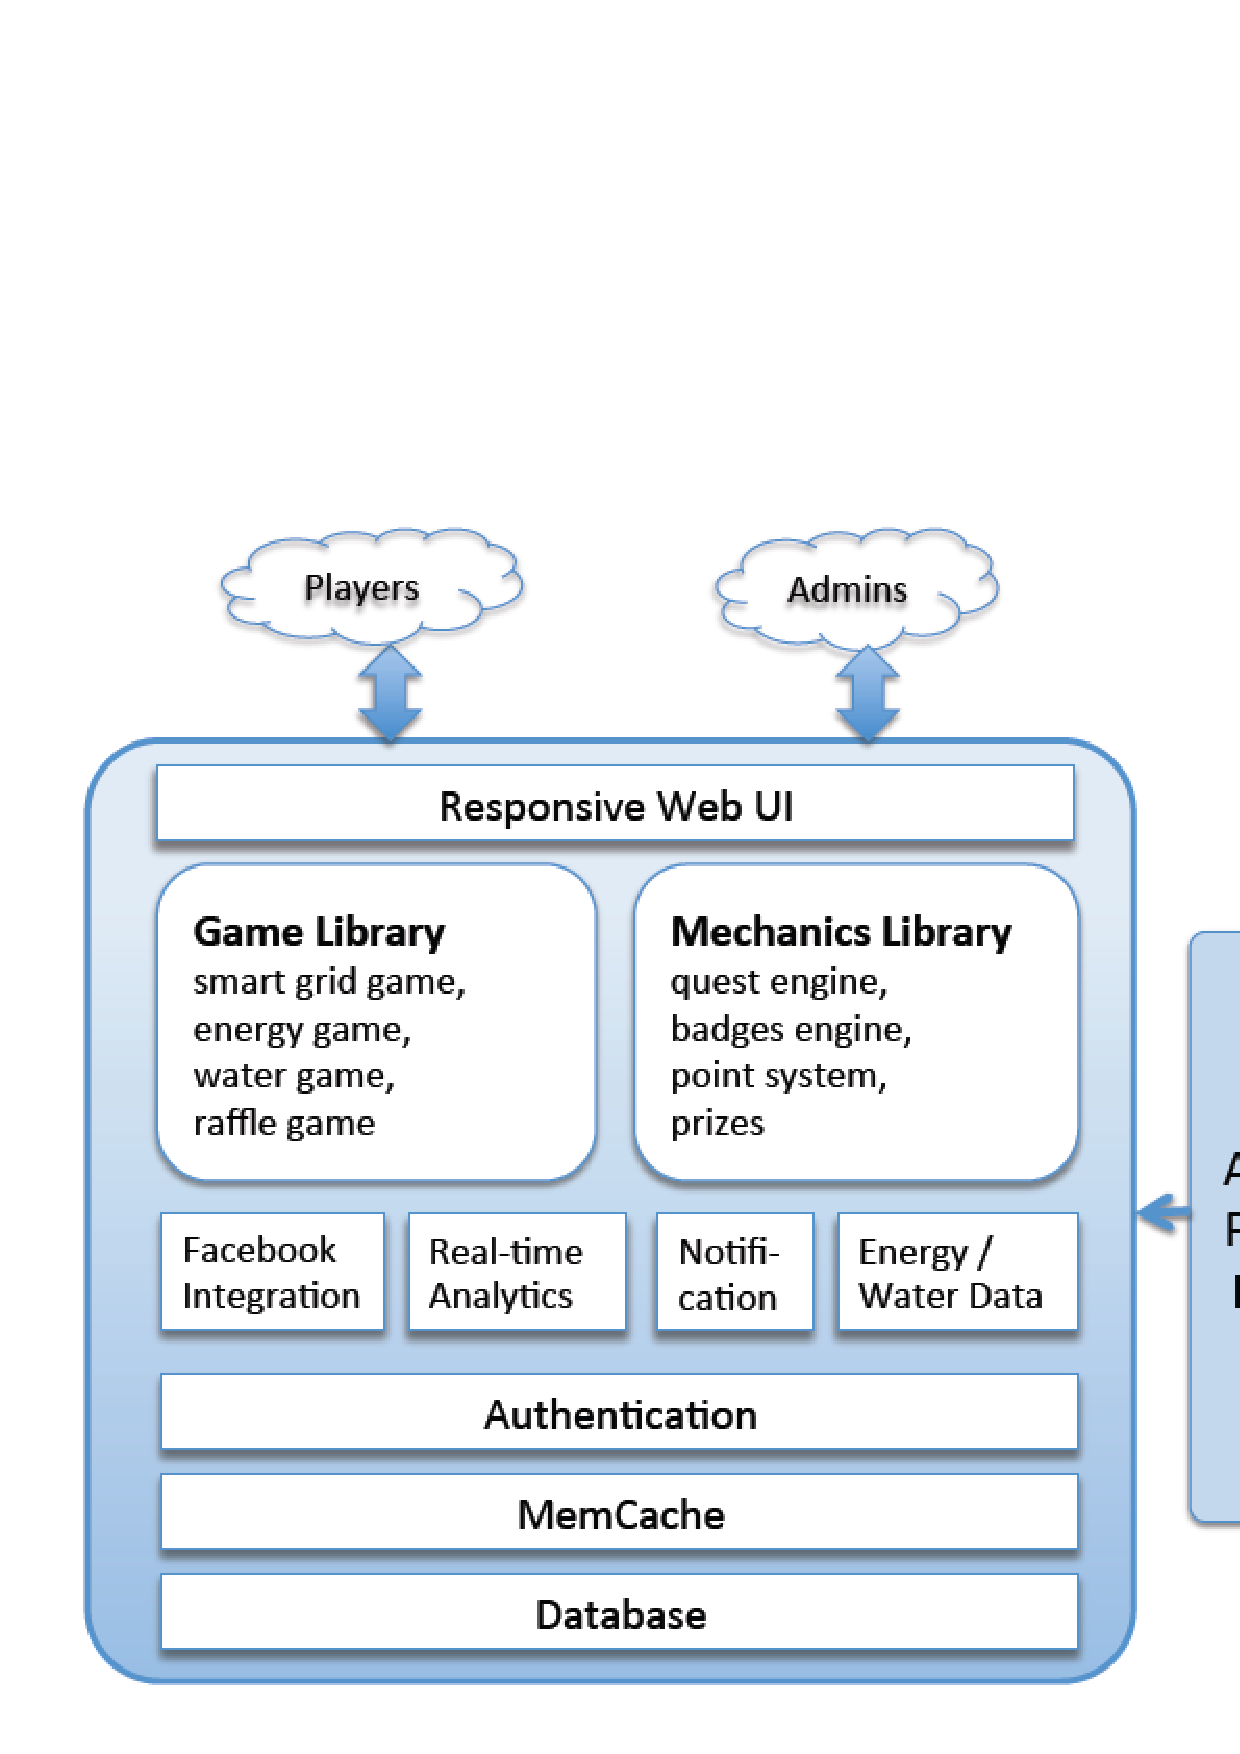
\includegraphics[width=\columnwidth]{makahiki-system-architecture}
  \caption{Architecture of Makahiki}
  \label{fig:makahiki-architecture}
\end{figure}

\begin{figure}
	\center
		\subfigure[Smart Grid Game]{\label{fig:SmartGrid}\includegraphics[width=0.48\columnwidth]{smart-grid-game.eps}}
		\subfigure[Energy Goal Game]{\label{fig:DailyEnergyGoal}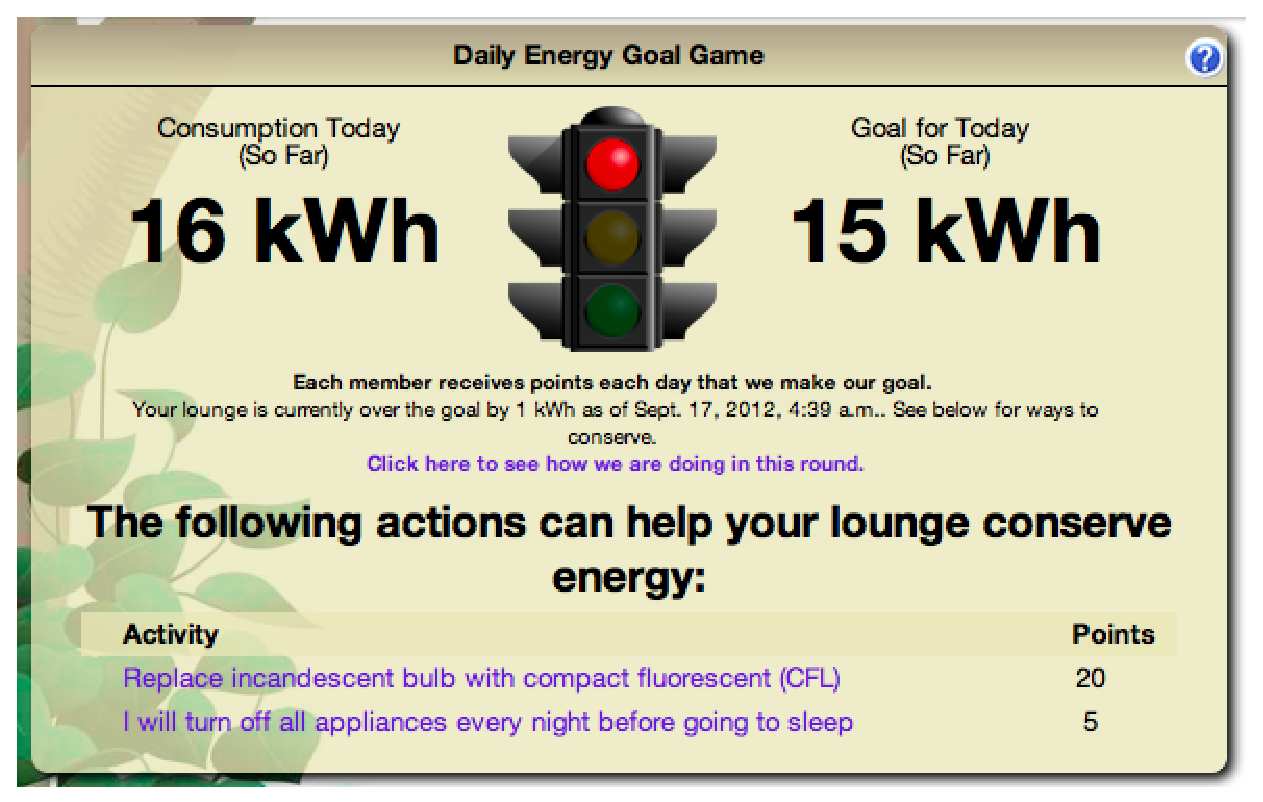
\includegraphics[width=0.48\columnwidth]{daily-energy-goal-game.eps}}
		\caption{Makahiki Game Library}
		\label{fig:makahiki-games}
\end{figure}

\subsection{Experiences with Makahiki}

We had used Makahiki to create four different Kukui
Cup Energy Challenges. Kukui Cup Energy challenges were held at the
University of Hawaii (UH) in 2011 and 2012 for over 1,000 first
year students living in the residence halls. Hawaii Pacific University
(HPU) held a Kukui Cup Energy challenge in Fall 2012 for about 200
students. An international organization called the East-West Center
(EWC) held a Kukui Cup Energy and Water challenge for the
international residents living in the residence halls without smart
meters, so the resource consumption data had to be entered by the game
mangers manually.

The successful creation of serious game challenges by three different organizations
provides four types of evidence that the Makahiki serious game framework can be tailored
to the needs of different organizations. First, UH and HPU used different metering
infrastructure, and EWC collected their resource data manually.  Second, while UH and HPU
challenges involved only energy consumption data, the EWC challenge involved both energy
and water consumption data. Third, the IT infrastructure at UH and HPU provided
authentication services using CAS (Central Authentication Service) and LDAP, while EWC
used the built-in Django authentication.  Fourth, the user interface was customized to
``brand'' each challenge with the logo, thematic elements, and the education contents of
the sponsoring organizations.

Besides the real world usage of Makahiki in the series of Kukui Cup challenges, we also
performed in-lab evaluation experiments. Makahiki was used in a serious game development
course in Spring semester of 2013 at the University of Hawaii Information and Computer Sciences department. There
were total 8 students that participated in the experiments. They were senior undergraduates
 or graduate students majoring in Computer Science. During the course, the students
installed Makahiki, configured and designed a serious game instance with Makahiki, and
finally developed an enhancement to the Makahiki framework. We asked the students taking
the course to voluntarily participate in the evaluation experiments of Makahiki, using
SGSEEM.

\subsection{Evaluation of Makahiki}

This section describes the details of Makahiki evaluation using SGSEEM. Some preliminary results are included here.

\subsubsection{Player Effectiveness Evaluation}

We evaluated player effectiveness using the 2011 Kukui Cup Challenge at
the University of Hawaii at Manoa. There were over 1000 eligible players
for this challenge, who were mostly first year college students living
in a cluster of four similar structured resident halls. Makahiki
recorded detailed logging data from every interaction between the
players and the website.

To assess the effectiveness in players' literacy in sustainability, we conducted
the two surveys, one before the challenge (pre-game) and
one after the challenge (post-game). The players' sustainability
literacy and behavior change was:
% CAM: need to put in some preliminary results.

To assess the effectiveness of positive player behavior changes in sustainability, the
energy consumption data before, during and after the challenge were
examined to understand any usage pattern or reduction during and after
the challenge. The results were:
% CAM: need to put in some preliminary results.

To assess the level of player engagement of the game, we calculated the engagement
metrics and the results were shown in \ref{fig:makahiki-engagement}:
\begin{figure}
  \centering
  \begin{tabular}{|c|c|}
    \hline
    \multicolumn{1}{|p{0.5\columnwidth}|}{\centering\tabhead{Measurement}} &
    \multicolumn{1}{|p{0.5\columnwidth}|}{\centering\tabhead{Value}} \\
    \hline
    \multicolumn{1}{|p{0.5\columnwidth}|}{Participation rate} &
    \multicolumn{1}{|p{0.5\columnwidth}|}{29} \\
    \hline
    \multicolumn{1}{|p{0.5\columnwidth}|}{Number of players per day (AVG, MAX, MIN)} &
    \multicolumn{1}{|p{0.5\columnwidth}|}{(40, 130, 1)} \\
    \hline
    \multicolumn{1}{|p{0.5\columnwidth}|}{Play time per day (AVG, MAX, MIN} &
    \multicolumn{1}{|p{0.5\columnwidth}|}{(15mins, 8.8hours, 1mins)} \\
    \hline
    \multicolumn{1}{|p{0.5\columnwidth}|}{submissions per day} &
    \multicolumn{1}{|p{0.5\columnwidth}|}{111} \\
    \hline
    \multicolumn{1}{|p{0.5\columnwidth}|}{social interaction per day} &
    \multicolumn{1}{|p{0.5\columnwidth}|}{101} \\
    \hline
  \end{tabular}
  \caption{Makahiki Engagement Metrics}
  \label{fig:makahiki-engagement}
\end{figure}

As we can see here, the participation rate is 29\% which is relatively high comparing to other sustainability challenges. over the course of the challenge, an average player spent average 15 minutes per day on the website. One player spent 8.8 hours in one of the days he played. There are 111 average serious game related activity submissions and 101 social interactions between players per day. This data provide an detailed insight about the high level of engagement of one of the Makahiki game instances.

\subsubsection{System Admin Efficiency Evaluation}

System admin efficiency evaluation was performed using the in-lab experiment.
Students in the serious game class were tasked with installing the Makahiki
system into their local computers as well as the cloud environment. In
order to understand how much time it takes to install the Makahiki and
what problems might be encountered, We designed two Google Forms which
details the steps of installing Makahiki both locally and in the
cloud, and for each step, we asked the students to record the time
they spent and the problems they encountered.

\autoref{fig:makahiki-eval-form} illustrates a partial Google Form
used for Makahiki system admin evaluation.

\begin{figure}[ht!]
   \centering
   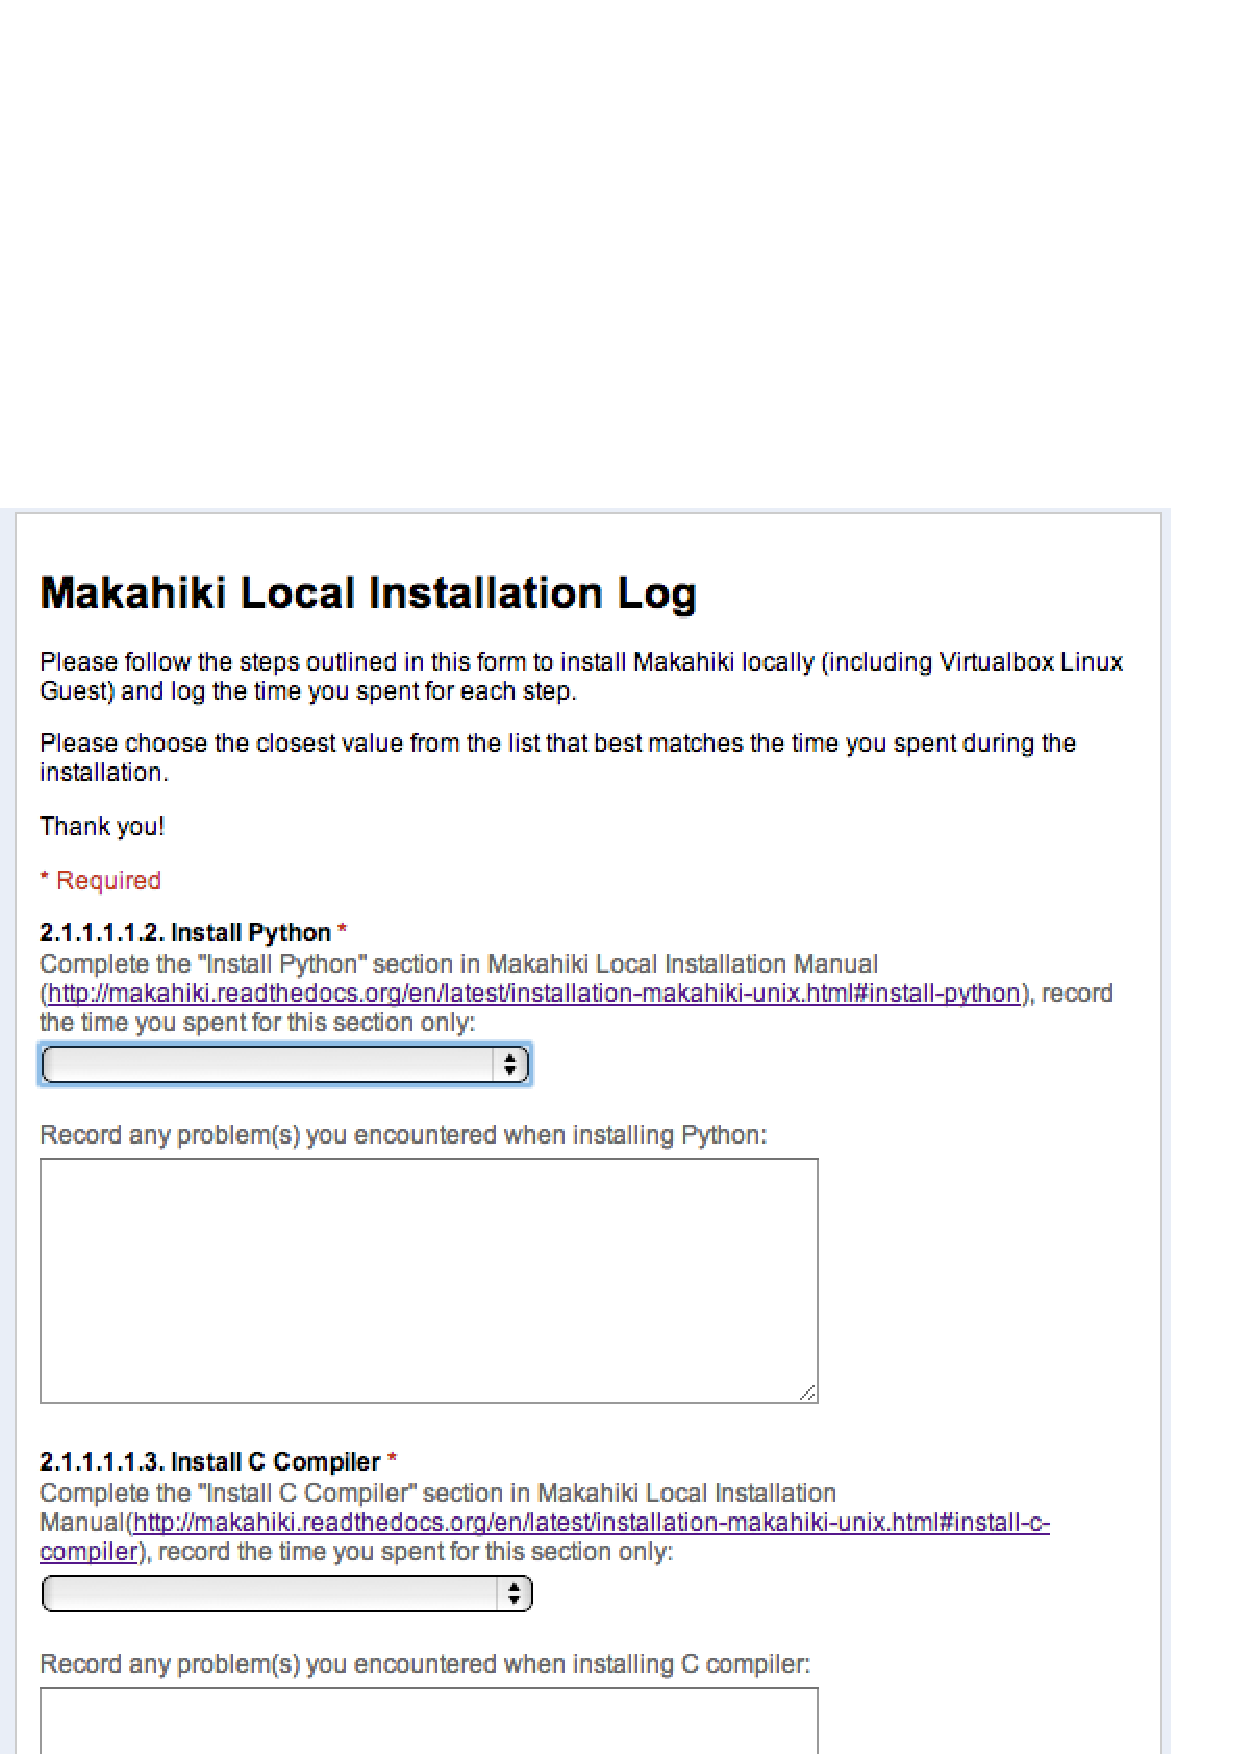
\includegraphics[width=\columnwidth]{developer-eval-form}
   \caption{Makahiki Evaluation Form}
   \label{fig:makahiki-eval-form}
\end{figure}

We also asked the students to provide feedback about their installation experiences
in the form of blog posts.


\subsubsection{Game Designer Efficiency Evaluation}

We used both the real world instances and in-lab experiment to evaluate the game
designer efficiency of Makahiki.

We interviewed the game designers of the Hawaii Pacific University challenge
 and the East-West Center challenge, asking questions outlined in the game designer
 experience section of the SGSEEM. We analyzed both the qualitative data collected from
the interviews and email exchanges, and the
quantitative data collected from the admin interface log data.

One of the class assignment for students in the in-lab experiment was to design a
Kukui-Cup-like serious game using Makahiki. We asked the students to follow specific
design steps and record the time required and any problems encountered during
their design process, using a Google Form similar to the one used for the system admin
evaluation. In addition, students were asked to provide feedback about their
design experiences in the form of blog posts.

% CAM: need to put in some preliminary results.

\subsubsection{Game Manager Efficiency Evaluation}

Game manager efficiency evaluation was performed by interviewing the
game managers of the Hawaii Pacific University and East-West Center at
Hawaii challenges. The interviews took place after the challenge. We
asked them about their experiences in using the Makahiki admin
interface for the managing process during the challenge. The admin
interface log data was also analyzed to assess if there were any errors
encountered during challenge management.
% CAM: need to put in some preliminary results.

\subsubsection{Developer Efficiency Evaluation}

In one of the assignments of the serious games class of the in-lab experiment,
the students were tasked with developing an enhancement to Makahiki. This
involved setting up a development environment, following the tutorial
to create a "Hello world" widget using Makahiki, and finally,
developing an enhancement which extended the functionality of Makahiki.

The students were asked to submit their development source code to the
public source code repository (GitHub) and write a blog post to
discuss their efforts to complete the development activity.

We reviewed their source code to compare their code to a reference
implementation, analyzed the blog posts from the students, as well as
any email correspondence from students discussing problems they encountered.
% CAM: need to put in some preliminary results.

\subsubsection{Researcher Efficiency Evaluation}

Several researchers in our department and another department are currently using
 Makahiki and the Kukui Cup challenge to do research on the areas of energy behavior
 changes and their motivations. As of the writing of this paper, we have not formally evaluate their experience regarding the role of researcher stakeholder. As one of
  the future work, We are planning to interview them and analyze the data as outlined
  in the the SGSEEM researcher experience efficiency section.

\section{Future Work}

The development of SGSEEM creates another research question:
what are the strengths and weaknesses of this evaluation method itself? To
answer this question, we are planing to apply SGSEEM
to another serious game framework.
%(such as the commercial Lucid Dashboard system~\cite{building-dashboard})
With the insights gained from another case study, SGSEEM can be further
improved.

One area of effectiveness evaluation that is currently not addressed in
SGSEEM: the longitudinal evaluation of player effectiveness. It would be
very useful to determine whether the serious game experience actually
had lasting impacts on players. In the context of Makahiki-based serious
games for sustainability, this would include things such as whether the
student players were able to continue any positive sustainability
behaviors after leaving their residence halls.

\section{Conclusion}

We have developed a serious game framework evaluation method called
Serious Game Stakeholder Experience Evaluation Method (SGSEEM). SGSEEM
evaluates serious game frameworks from the perspective of different
stakeholders' experiences: player effectiveness, system administrator efficiency,
game designer efficiency, game manager efficiency,
developer efficiency, and researcher efficiency. These experiences are
evaluated qualitatively and quantitatively to determine the extent of effectiveness
 and efficiency of a serious game framework.

We also applied SGSEEM to Makahiki. The preliminary results of the evaluation show
that: a) Makahiki is effective from players' perspective in the ways of increase
 in player sustainability literacy, decrease in energy consumption, and engaging
 players, b) Makahiki is relatively easy to install from a system administrator's
 perspective, c) Makahiki has rooms for improvement in the efficiency of a game
 designer, d) Makahiki is relatively easy to manage from a game manager's perspective,
  e) Makahiki could be improved by providing better support for developers.

\section{Acknowledgments}
Omitted from review version.

%\textbf{Don't forget
%to acknowledge funding sources as well}, so you don't wind up
%having to correct it later.

% Balancing columns in a ref list is a bit of a pain because you
% either use a hack like flushend or balance, or manually insert
% a column break.  http://www.tex.ac.uk/cgi-bin/texfaq2html?label=balance
% multicols doesn't work because we're already in two-column mode,
% and flushend isn't awesome, so I choose balance.  See this
% for more info: http://cs.brown.edu/system/software/latex/doc/balance.pdf
%
% Note that in a perfect world balance wants to be in the first
% column of the last page.
%
% If balance doesn't work for you, you can remove that and
% hard-code a column break into the bbl file right before you
% submit:
%
% http://stackoverflow.com/questions/2149854/how-to-manually-equalize-columns-
% in-an-ieee-paper-if-using-bibtex
%
% Or, just remove \balance and give up on balancing the last page.
%
\balance

% If you want to use smaller typesetting for the reference list,
% uncomment the following line:
% \small
\bibliographystyle{acm-sigchi}
\bibliography{sustainability,csdl-trs,gamification,13-03}
\end{document}
